%% LyX 2.2.3 created this file.  For more info, see http://www.lyx.org/.
%% Do not edit unless you really know what you are doing.
\documentclass[9pt,twocolumn,brazil]{article}
\usepackage[T1]{fontenc}
\usepackage[utf8]{inputenc}
\usepackage{fancyhdr}
\usepackage{graphicx}
\usepackage{amsmath}
\usepackage{geometry}
%%%%% GENEXAMS SPECIFIC %%%%%%%%%%%%
\mathcode`,="002C
\usepackage{tabularx}
%\usepackage[locale=FR]{siunitx}
%\sisetup{per-mode=symbol}
\geometry{verbose,tmargin=1cm,bmargin=2cm,lmargin=1cm,rmargin=1cm}
\usepackage{xcolor,colortbl}
\definecolor{black}{rgb}{0,0,0}
\newcommand{\black}{\cellcolor{black}}  %{0.9}

\makeatletter
%%%%%%%%%%%%%%%%%%%%%%%%%%%%%% User specified LaTeX commands.
\usepackage{setspace}
\usepackage[sort]{cite}
%\pagestyle{empty}
\pagestyle{fancy}
\fancyhead{}
\fancyfoot{}
\renewcommand{\headrulewidth}{0.0pt}
\fancyfoot[RO,RE]{2/2022.11.22-15.18.49}

\makeatother

\usepackage{babel}
\begin{document}

\textbf{Universidade Federal de Ouro Preto}

\textbf{Instituto de Ciências Exatas e Biológicas}

\textbf{Departamento de Física}

\textbf{Prof. Dr. Alan Barros de Oliveira}\\

Prova 2 -- FIS110-73 -- 17/06/2022\medskip{}

%\textbf{Considere a aceleração gravitacional $g=\SI{9.8}{\meter\per\square\second}$}\medskip{}



1. Considere um corpo de massa $m$, sob a ação de um campo de forças $F$ conservativo, cuja energia mec\^anica \'e $E=K+U$, onde $K$ e $U$ s\~ao as energias cin\'etica e potencial. Considerando que o movimento do corpo é restrito a uma dimensão, pode-se afirmar que\\
(a) se $K<0$ o sistema atinge o equilíbrio indiferente.\\
(b) $F=-dU/dx$.\\
(c) $K=U$ apenas em pontos de retorno.\\
(d) se $F=mg$ o sistema encontra-se em repouso ultra-móvel.\\
(e) Todas as outras alternativas são falsas.\\

2. Uma part\'{i}cula de massa 2,1 kg, lan\c cada sobre um trilho retil\'{i}neo com velocidade de 3,6 m/s, est\'a sujeita a uma for\c ca $F(x) = -bx$, onde $b=1,0$ N/m e $x$ \'e o deslocamento, em m, a partir da origem. Sabendo-se que a part\'icula para em dois pontos do trilho, a saber, $+x_0$ e $-x_0$, determine $x_0$ em metros.\\
(a)5,2~
(b)1,4~
(c)11,4~
(d)7,5~
(e)9,2\\

3. Na figura abaixo, um pequeno bloco de 87 g desliza para baixo em uma superfície curva sem atrito a partir de uma altura $h=29$ cm e depois adere a uma barra uniforme de massa 142 g e comprimento 79 cm. A barra gira em torno do ponto O antes de parar  momentaneamente. Determine $\theta$ em graus.\\
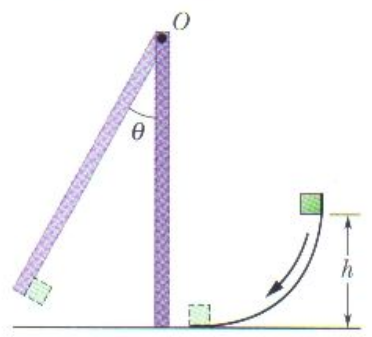
\includegraphics[width=4.0cm]{../input/figs/fig1}\\
(a)34,9~
(b)9,4~
(c)19,7~
(d)29,6~
(e)0,4\\

4. A figura abaixo mostra um corpo rígido formado por um aro fino (de massa $m$, raio $R=$ 0,44 m e momento de inércia em relação ao diâmetro $mR^2/2$) e uma barra fina radial (de massa $m$,  comprimento $L=2,00R$ e momento de inércia em relação ao seu CM $mL^2/12$). O conjunto está na vertical, mas se recebe um pequeno empurrão começa a girar em torno de um eixo horizontal no plano do aro e da barra, que passa pela extremidade inferior da barra. Supondo que a energia fornecida ao sistema pelo pequeno empurrão é desprezível, qual é a velocidade angular em rad/s do conjunto quando ele passa pela posição invertida (de cabeça para baixo)?\\
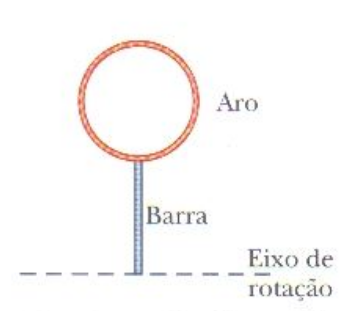
\includegraphics[width=4.0cm]{../input/figs/fig-10-65}\\
(a)10,94~
(b)5,79~
(c)6,90~
(d)8,31~
(e)3,61\\

5. Considere um objeto que se move em uma dimens\~ao de acordo com a equa\c c\~ao hor\'aria $x=v_0 t e^{-t/t_0}$, onde $t$ \'e o tempo, $v_0 = 11,1$ m/s  e $t_0 = 1,3$ s. Qual \'e a dist\^ancia, em metros, que o objeto se encontra da origem quando para momentaneamente?\\
(a)5,3~
(b)7,2~
(c)12,0~
(d)8,2~
(e)11,0\\

6. Uma pequena aranha de peso $P_a$ está pendurada na ponta de um fio de teia, no teto de um elevador. Sabendo-se que o fio suporta uma tensão máxima de $5,8P_a$, qual seria a mínima aceleração (em m/s$^2$) de subida do elevador para que o fio se partisse?\\
(a)15,8~
(b)59,3~
(c)48,0~
(d)28,2~
(e)74,3\\

7. Duas partículas, de massas $m_1$ e $m_2$, são empurradas uma contra a outra, comprimindo uma mola colocada entre elas. Quando são liberadas, a mola as arremessa em sentidos opostos. A relação entre as massas das partículas é $m_2/m_1 = 3$ e a energia armazenada na mola é de 78 J. Suponha que a mola tenha massa desprezível e que toda a energia armazenada seja transferida para as partículas. Após terminada essa transferência, qual é a energia cinética \textbf{da partícula 1} em J?\\
(a)58,5~
(b)14,7~
(c)22,9~
(d)35,8~
(e)46,6\\

8. Considere uma colis\~ao frontal el\'astica entre duas part\'{i}culas de massas $m$ e $m^{\prime}=10m$. A part\'{i}cula de massa $m$ se move inicialmente com velocidade $v$, enquanto a outra encontra-se em repouso. Qual é a fra\c c\~ao de energia cin\'etica transferida de $m$ para $m^{\prime}$ durante a colisão?\\
(a)0,33~
(b)0,04~
(c)0,43~
(d)0,63~
(e)0,88\\

9. Um metrô percorre uma curva plana de raio 9 m a 17 km/h. Qual o ângulo, em graus, que as alças de mão penduradas no teto fazem com a vertical?\\
(a)62,9~
(b)77,2~
(c)48,2~
(d)72,7~
(e)39,6\\

10. Um rifle, que atira balas a 423 m/s, é apontado para um alvo situado a 51 m de distância. Se o centro do alvo está na mesma altura do rifle, para que altura (\textbf{em centímetros}) acima do alvo o cano do rifle deve ser apontado para que a bala atinja o seu centro?\\
(a)32,5~
(b)7,3~
(c)103,2~
(d)70,8~
(e)58,0\\


%\noindent\rule{6cm}{0.7pt}\\
{\large \textbf{Fórmulas e Constantes}}
\begin{align*}
%-----------CHAP. 33 and 35-------------
	%&E=E_m\sin(kx-\omega t);~~B=B_m\sin(kx-\omega t)&\\
	%&c=\frac{E}{B}=\frac{E_m}{B_m}={\sqrt{\mu_0 \epsilon_0}};~~\vec{S}=\frac{1}{\mu_0}\vec{E}\times\vec{B}&\\
	%&I=\frac{1}{c\mu_0}\frac{E_m^2}{2};~~I=\frac{P_s}{4\pi r^2};~~P_r=\frac{F}{A}=\gamma\frac{I}{c}~(\mathrm{onde}~1\leq\gamma\leq2)&\\
	%&I=\frac{I_0}{2};~~I=I_0 \cos^2\theta;~~n_1\sin\theta_1=n_2\sin\theta_2~~&\\
	%&\theta_c=\sin^{-1}\frac{n_2}{n_1};~~\theta_B=\tan^{-1}\frac{n_2}{n_1};~~\lambda_n = \frac{\lambda}{n};~~n=\frac{c}{v};~~v=f\lambda&\\
%-----------CHAP. 38 and 39-------------
	&I=\frac{P_s}{4\pi r^2};~~E=hf;~~p=\frac{hf}{c}=\frac{h}{\lambda}&\\
	&hf=K_\mathrm{max}+\Phi;~~\Delta\lambda=\frac{h}{mc}(1-\cos\phi)&\\
	&\frac{d^2\psi}{dx^2}+\frac{8\pi^2 m}{h^2}[E-U(x)]\psi=0&\\
	&T\approx e^{-2bL},~\mathrm{onde}~b=\sqrt{\frac{8\pi^2 m(U_b-E)}{h^2}}&\\
	&E_n=\left(\frac{h^2}{8mL^2}\right)n^2,~\mathrm{para}~n=1,2,3\dots&\\
	&\psi_n(x)=A\sin\left(\frac{n\pi}{L}x\right),~\mathrm{para}~n=1,2,3\dots&\\
	&\Delta x \Delta p = h/2\pi&\\
%--------CONSTANTS----------------------
	&\epsilon_0 = 8,854\times10^{12}~\mathrm{F/m};~~\mu_0 = 1,257\times10^{-6}~\mathrm{H/m}&\\
	&c=3,0\times10^8~\mathrm{m/s};~~h=6,63\times10^{-34}~\mathrm{J/s}=4,14\times10^{-15}~\mathrm{eV.s}&\\
	&hc=1240~\mathrm{eV.nm}&\\
	&\mathrm{Eletron:}~~mc^2 = 511~\mathrm{keV}&\\
%---------------------------------------
\end{align*}
%\rule{6cm}{0.7pt}
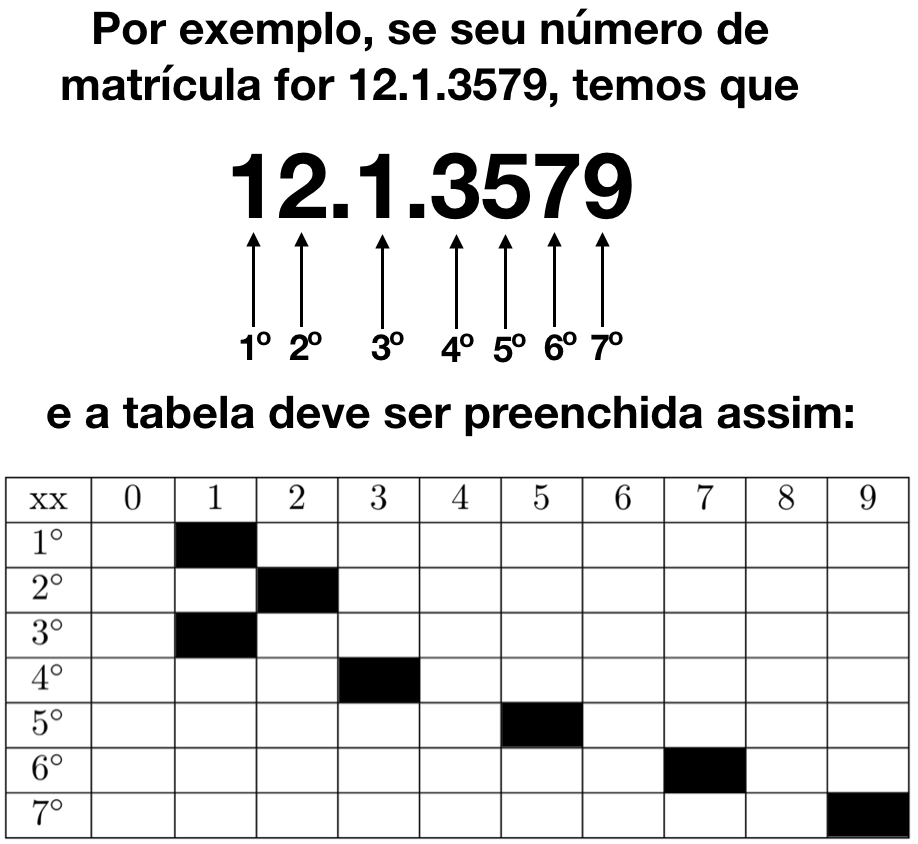
\includegraphics[width=6cm]{../aux/matricula.png}\\
\vfill
\pagebreak
\begin{tabular}{!{\vrule width 1.5pt}c|c|c|c|c|c|c|c|c|c|c!{\vrule width 1.5pt}}
\noalign{\hrule height 1.5pt}
	\multicolumn{1}{!{\vrule width 1.5pt}c}{} & \multicolumn{9}{c}{\textbf{NÃO MARCAR}} & \tabularnewline
\hline 
un&--&--&\black&--&--&--&--&--&--&-- \tabularnewline
\hline%un 
%--&--&--&--&--&--&--&--&--&-- \tabularnewline
 
%--&--&--&--&--&--&--&--&--&--  \tabularnewline
 
	\multicolumn{1}{!{\vrule width 1.5pt}c}{} & \multicolumn{9}{c}{\textbf{GABARITO}} &  \tabularnewline
\hline
-- & 1 & 2 & 3 & 4 & 5 & 6 & 7 & 8 & 9 & 10\tabularnewline
\hline
a &   &   &   &   &   &   &   &   &   &  \tabularnewline
\hline
b &   &   &   &   &   &   &   &   &   &  \tabularnewline
\hline
c &   &   &   &   &   &   &   &   &   &  \tabularnewline
\hline
d &   &   &   &   &   &   &   &   &   &  \tabularnewline
\hline
e &   &   &   &   &   &   &   &   &   &  \tabularnewline
\hline
\multicolumn{1}{!{\vrule width 1.5pt}c}{} & \multicolumn{9}{c}{\textbf{MATRÍCULA}} & \tabularnewline
\hline 
-- & \phantom{0}0 & \phantom{0}1 & \phantom{0}2 & \phantom{0}3 & \phantom{0}4 & \phantom{0}5 
& \phantom{0}6 & \phantom{0}7 & \phantom{0}8 & \phantom{0}9\tabularnewline
\hline 
1$^{\circ}$ &  &  &  &  &  &  &  &  &  & \tabularnewline
\hline 
2$^{\circ}$ &  &  &  &  &  &  &  &  &  & \tabularnewline
\hline 
3$^{\circ}$ &  &  &  &  &  &  &  &  &  & \tabularnewline
\hline 
4$^{\circ}$ &  &  &  &  &  &  &  &  &  & \tabularnewline
\hline 
5$^{\circ}$ &  &  &  &  &  &  &  &  &  & \tabularnewline
\hline 
6$^{\circ}$ &  &  &  &  &  &  &  &  &  & \tabularnewline
\hline 
7$^{\circ}$ &  &  &  &  &  &  &  &  &  & \tabularnewline
\noalign{\hrule height 1.5pt}
\end{tabular}
\vfill

\textbf{MATRÍCULA:}

\vspace{0.5cm}

\textbf{NOME:}

\vspace{0.5cm}

\textbf{TURMA:}
\end{document}